%\documentclass[12pt,preprint]{aastex}
\documentclass[12pt,preprint]{emulateapj}
\usepackage{graphicx}

%% read tex files
%%\input{newcommand_gen.tex} % general commands
%%\input{planetinfo_156846.tex} % parameter values for HD 97658 b


\shorttitle{Transit Search for HD~168443b\lowercase{b}}
\shortauthors{Pilyavsky et al.}
\slugcomment{Submitted for publication in the Astrophysical Journal}
%\received{2007 November 09}

\begin{document}

\title{A Search for the Transit of HD~168443\lowercase{b}: Improved Orbital Parameters and Photometry }

\author{
  Genady Pilyavsky\altaffilmark{1},
  Suvrath Mahadevan\altaffilmark{1},
  Stephen R. Kane\altaffilmark{2},
  Andrew W. Howard\altaffilmark{3,4},
  Kaspar von Braun\altaffilmark{2},
  David R. Ciardi\altaffilmark{2},
  Diana Dragomir\altaffilmark{5},
  Debra Fischer\altaffilmark{6},
  Gregory W. Henry\altaffilmark{7},
  Greg Laughlin\altaffilmark{9},
  Markus Rabus\altaffilmark{10},
  Jason Wright\altaffilmark{1}
}
\email{suvrath@astro.psu.edu}
\altaffiltext{1}{Department of Astronomy and Astrophysics,
  Pennsylvania State University, 525 Davey Laboratory, University
  Park, PA 16802}
\altaffiltext{2}{NASA Exoplanet Science Institute, Caltech, MS 100-22,
  770 South Wilson Avenue, Pasadena, CA 91125}
\altaffiltext{3}{Department of Astronomy, University of California,
  Berkeley, CA 94720}
\altaffiltext{4}{Space Sciences Laboratory, University of California,
  Berkeley, CA 94720}
\altaffiltext{5}{Department of Physics \& Astronomy, University of
  British Columbia, Vancouver, BC V6T1Z1, Canada}
\altaffiltext{6}{Department of Astronomy, Yale University, New Haven,
  CT 06511}
\altaffiltext{7}{Center of Excellence in Information Systems, Tennessee
  State University, 3500 John A. Merritt Blvd., Box 9501, Nashville,
  TN 37209}
\altaffiltext{9}{UCO/Lick Observatory, University of California, Santa
  Cruz, CA 95064}
\altaffiltext{10}{Departamento de Astonom\'ia y Astrof\'isica,
  Pontificia Universidad Cat\'olica de Chile, Casilla 306, Santiago
  22, Chile}


%%%%%%%%%%%%%%%%%%%%%%%%%%%%%%%%%%%%%%%%%%%%%%%%%%%%%%%%%%%%%%%%%%%%

\begin{abstract}

HD~168443b
\end{abstract}

\keywords{planetary systems -- techniques: photometric -- techniques:
  radial velocities -- stars: individual (HD~168443)}

%%%%%%%%%%%%%%%%%%%%%%%%%%%%%%%%%%%%%%%%%%%%%%%%%%%%%%%%%%%%%%%%%%%%

\section{Introduction}
\label{introduction}

%%%%%%%%%%%%%%%%%%%%%%%%%%%%%%%%%%%%%%%%%%%%%%%%%%%%%%%%%%%%%%%%%%%%

\section{Why HD168443 is interesting}
\label{motivation}

%%%%%%%%%%%%%%%%%%%%%%%%%%%%%%%%%%%%%%%%%%%%%%%%%%%%%%%%%%%%%%%%%%%%

\section{Radial Velocity Measurements and Revised Orbital Parameters}
\label{revisedop}

%%%%%%%%%%%%%%%%%%%%%%%%%%%%%%%%%%%%%%%%%%%%%%%%%%%%%%%%%%%%%%%%%%%%

\subsection{Observations}


\subsection{Stellar Properties}
\label{steprop}



%%%%%%%%%%%%%%%%%%%%%%%%%%%%%%%%%%%%%%%%%%%%%%%%%%%%%%%%%%%%%%%%%%%%

\subsection{Keplerian Models}





%%%%%%%%%%%%%%%%%%%%%%%%%%%%%%%%%%%%%%%%%%%%%%%%%%%%%%%%%%%%%%%%%%%%

\section{Transit Ephemeris Refinement}
\label{ephemeris}


%%%%%%%%%%%%%%%%%%%%%%%%%%%%%%%%%%%%%%%%%%%%%%%%%%%%%%%%%%%%%%%%%%%%

\section{Hipparchos Photometry of HD168443}
The Hipparchos mission observed the brightest stars in the sky over many epochs. \citet{Robichon00} and \citet{Castellano00} detected the transit of HD209458b in the Hipparchos epoch photometry, and \citet{Hebrard06} were able to detect multiple transits of HD189733b, leading to a significant improvement in the determination of its period.  Hipparchos photometry has therefore been demonstrated to be precise enought to detect the transit of a Jupiter radii planet around stars fainter than HD168443 (V=6.92).  Figure \ref{fig:hip} shows the Hipparchos photometry and phasing on the known period for HD209458 and for the period we derived from long term radial velocity monitoring in section \ref{ephemeris} for HD168443. We follow the prescription of \citet{Robichon00} to create the phased plot. A long period planet, like HD168443b, has a significantly smaller probablilty (than a few day period hot Jupiter) of a Hipparchos observational epoch corresponding to a transit. 

\begin{figure}[h]
  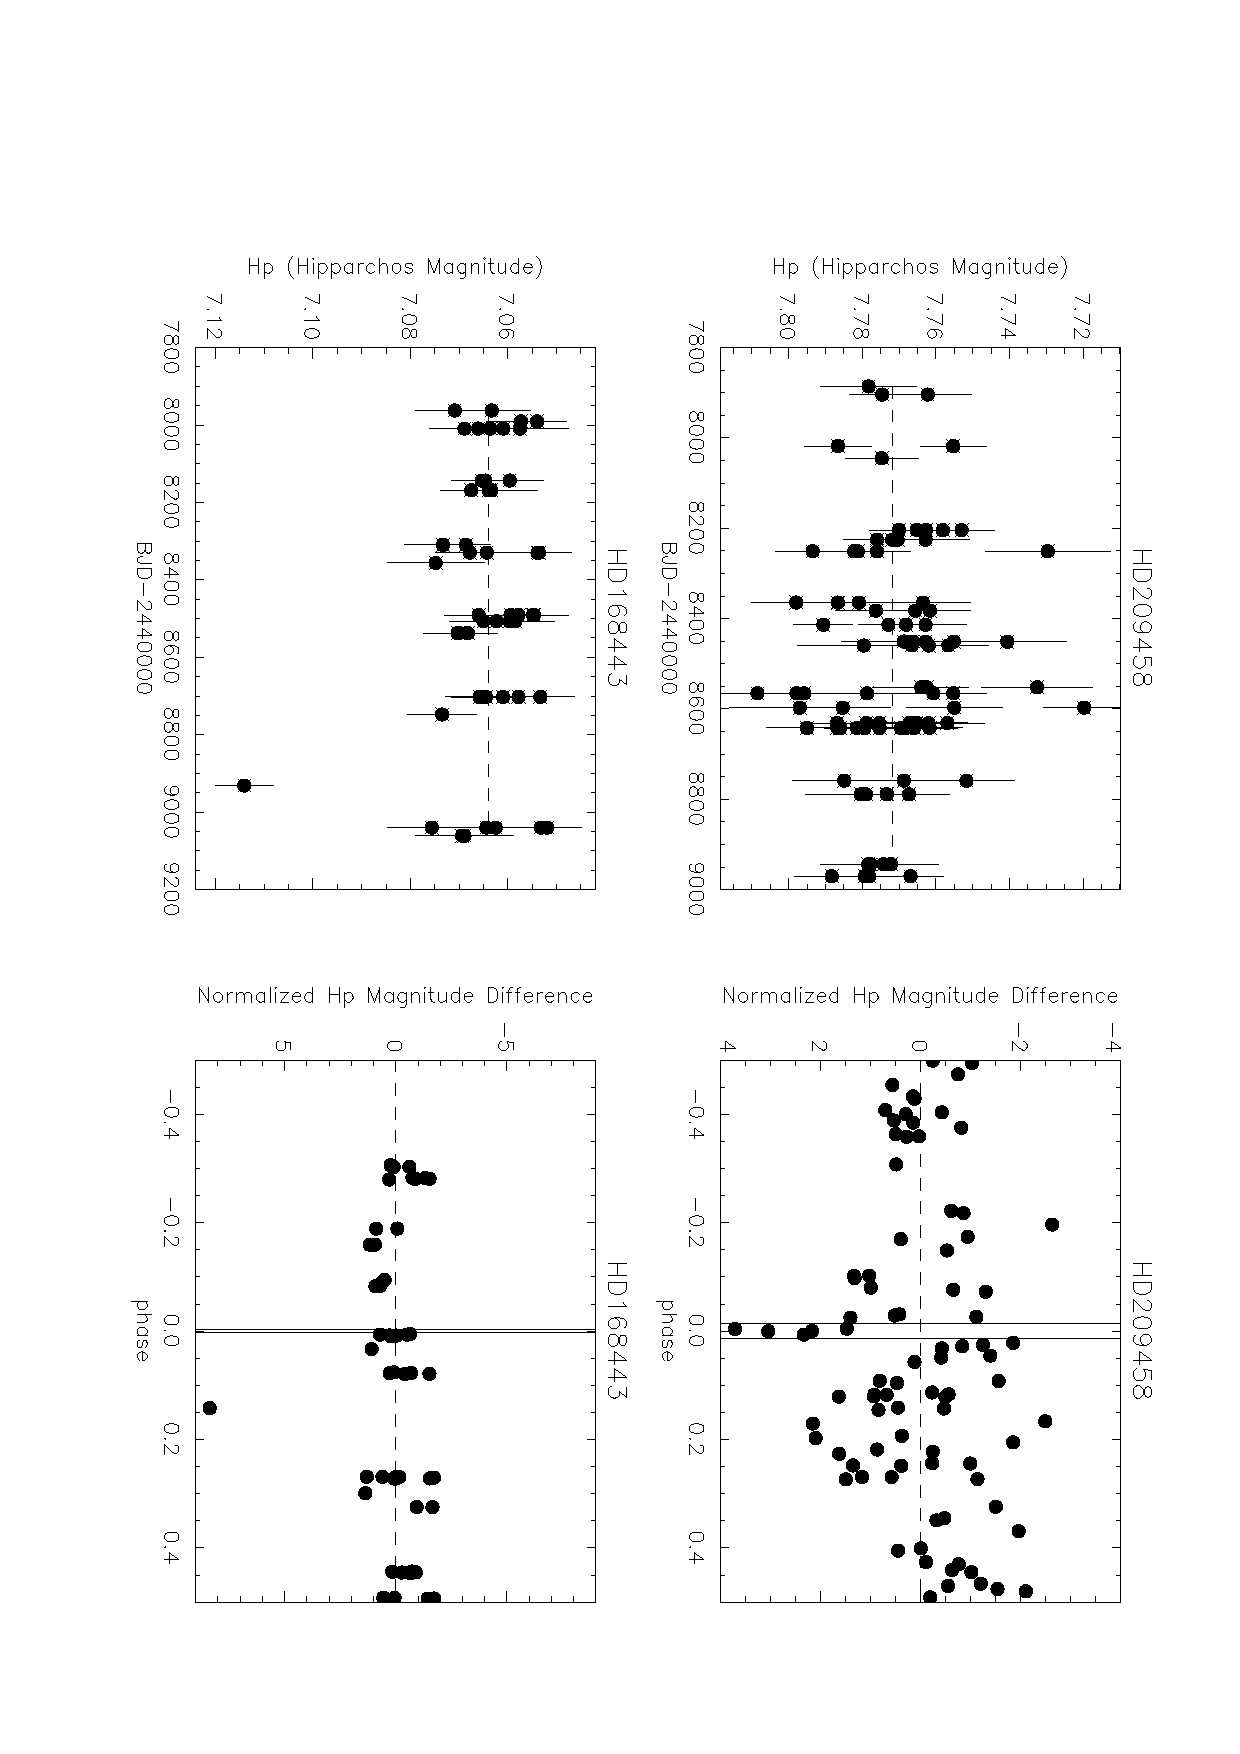
\includegraphics[angle=90,width=8.2cm]{HipparcosCheck}
  \caption{Hipparchos Photometry}
  \label{fig:hip}
\end{figure}


%%%%%%%%%%%%%%%%%%%%%%%%%%%%%%%%%%%%%%%%%%%%%%%%%%%%%%%%%%%%%%%%%%%%

\section{Monitoring the Transit Window}
\subsection{CTIO Photometry}
\label{sec:photometry}

Since the PSF of the stars within each frame were non-gaussian in
shape, aperture photometry was used to measure each of the stars of
interest. For each star, a small part of the image ($\pm$~100 pixels
from the estimated center) was extracted from the frame. Estimates of
the extent of the PSF with suitable values for sky radii were then
passed to the photometry code for analysis. Due to the extreme
defocussing and stable guiding of the telescope, we found the
photometry to be relatively robust against the choice of these values.

As mentioned in Section \ref{sec:observing}, observing conditions on
the night of the transit window (2009 September 3) were not optimal
and plagued with thin cirrus. We were unfortunately unable to utilise
the bright reference stars in the alternate fields due to these
variable conditions. The difficulties imposed for this photometry thus
became dominated by the lack of bright reference stars within the 20
arcmin FOV. We selected the brightest four reference stars in the
frame which were $\sim 5$ magnitudes fainter than the target. Relative
photometry was performed using the methods described in \citet{eve01}.

\begin{figure}
 % \includegraphics[angle=270,width=8.2cm]{f03a.ps}
  %\includegraphics[angle=270,width=8.2cm]{f03b.ps}
  %\includegraphics[angle=270,width=8.2cm]{f03c.ps}
  \caption{CTIO photometry of HD~156846. Top: Data from 2009 September
    3 calibrated with four reference stars in the field, in which
    cloud effects are still present. Middle: Data from 2009 September
    3 calibrated with only the brightest reference star, corrected
    for airmass, and sigma-clipped. Bottom: For comparison, data from
    2009 September 9 using the same bright reference star and
    sigma-clipped, but no airmass correction is needed.}
  \label{fig:phot1}
\end{figure}

Shown in the top panel of Figure \ref{fig:phot1} is the lightcurve of
HD~156846 from the night of the transit window, calibrated using the
faint reference stars. The dip in the middle of the lightcurve is due
to cloud effects which are also present in the lightcurves of the
reference stars. The upward trend in the lightcurve is due to the
increasing airmass as the target was observed until it set. It was
found that only using the brightest reference star produced an
improved result in correcting for cloud effects. The lightcurve shown
in the middle panel of Figure \ref{fig:phot1} uses the brightest
reference star for calibration. A power law was applied to correct for
airmass, and a sigma-clip was performed to remove significant
outliers. The 1$\sigma$ scatter of the measurements in this panel is
slightly less than 1\%. For comparison, we show a lightcurve in the
bottom panel from the night of 2009 September 9 during which
conditions were significantly improved. This lightcurve uses the same
reference star but no airmass correction was needed or used. The
scatter is half that of the night of the transit window.

\subsection{APT Photometry}
%%%%%%%%%%%%%%%%%%%%%%%%%%%%%%%%%%%%%%%%%%%%%%%%%%%%%%%%%%%%%%%%%%%%

\section{Conclusions}

This stoopid object is not transiting either. Damn!

%%%%%%%%%%%%%%%%%%%%%%%%%%%%%%%%%%%%%%%%%%%%%%%%%%%%%%%%%%%%%%%%%%%%

\section*{Acknowledgements}

The authors would like to thank the anonymous referee, whose comments
greatly improved the quality of the paper. This work made use of the
SIMBAD database (operated at CDS, Strasbourg, France), NASA's
Astrophysics Data System Bibliographic Services, and the NASA Star and
Exoplanet Database (NStED). This work was partially supported by
funding from the Center for Exoplanets and Habitable Worlds. The
Center for Exoplanets and Habitable Worlds is supported by the
Pennsylvania State University, the Eberly College of Science, and the
Pennsylvania Space Grant Consortium. Finally, the authors wish to
extend special thanks to those of Hawai`ian ancestry on whose sacred
mountain of Mauna Kea we are privileged to be guests. Without their
generous hospitality, the Keck observations presented herein would not
have been possible.

%%%%%%%%%%%%%%%%%%%%%%%%%%%%%%%%%%%%%%%%%%%%%%%%%%%%%%%%%%%%%%%%%%%%

\begin{thebibliography}{}
\bibitem[Castellano et al.(2000)]{Castellano00} Castellano, T., 
Jenkins, J., Trilling, D.~E., Doyle, L., \& Koch, D.\ 2000, \apjl, 532, L51 
\bibitem[H{\'e}brard 
\& Lecavelier Des Etangs(2006)]{Hebrard06} H{\'e}brard, G., \& Lecavelier Des Etangs, A.\ 2006, \aap, 445, 341 
\bibitem[Robichon \& Arenou(2000)]{Robichon00} Robichon, N., \& Arenou, F.\ 2000, \aap, 355, 295 



\bibitem[\protect\citeauthoryear{Bakos et al.}{2004}]{bak04} Bakos,
  G., Noyes, R.W., Kov\'acs, G., Stanek, K.Z., Sasselov, D.D., Domsa,
  I., 2004, PASP, 116, 266
\bibitem[\protect\citeauthoryear{Barbieri et al.}{2007}]{bar07}
  Barbieri, M., et al., 2007, A\&A, 476, L13
\bibitem[\protect\citeauthoryear{Barge et al.}{2008}]{bar08}
  Barge, P., et al., 2008, A\&A, 482, L17
\bibitem[\protect\citeauthoryear{Barnes \& O'Brien}{2002}]{bar02}
  Barnes, J.W., O'Brien, D.P., 2002, ApJ, 575, 1087
\bibitem[\protect\citeauthoryear{Bodenheimer et al.}{2003}]{bod03}
  Bodenheimer, P., Laughlin, G., Lin, D.N.C., 2003, ApJ, 592, 555
\bibitem[\protect\citeauthoryear{Borucki et al.}{2010}]{bor10}
  Borucki, W.J., et al., 2010, Science, 327, 977
\bibitem[\protect\citeauthoryear{Butler et al.}{1996}]{but96} Butler,
  R.P., Marcy, G.W., Williams, E., McCarthy, C., Dosanjh, P., Vogt,
  S.S., 1996, PASP, 108, 500
\bibitem[\protect\citeauthoryear{Charbonneau et al.}{2000}]{cha00}
  Charbonneau, D., Brown, T.M., Latham, D.W., Mayor, M., 2000, ApJ,
  529, L45
\bibitem[\protect\citeauthoryear{Croll et al.}{2007}]{cro07} Croll,
  B., et al., 2007, ApJ, 658, 1328
\bibitem[\protect\citeauthoryear{Deeg et al.}{2010}]{dee10}
  Deeg, H.J., et al., 2010, Nature, 464, 384
\bibitem[\protect\citeauthoryear{Demarque et al.}{2004}]{dem04}
  Demarque, P., Woo., J., Kim, Y., Yi, S.K., 2004, ApJS, 155, 667
\bibitem[\protect\citeauthoryear{Everett \& Howell}{2001}]{eve01}
  Everett, M.E., Howell, S.B., 2001, PASP, 113, 1428
\bibitem[\protect\citeauthoryear{Fortney et al.}{2007}]{for07}
  Fortney, J.J., Marley, M.S., Barnes, J.W., 2007, ApJ, 659, 1661
\bibitem[\protect\citeauthoryear{Fortney et al.}{2010}]{for10}
  Fortney, J.J., Shabram, M., Showman, A.P., Lian, Y., Freedman,
  R.S., Marley, M.S., Lewis, N.K., 2010, ApJ, 709, 1396
\bibitem[\protect\citeauthoryear{Gillon et al.}{2007}]{gil07} Gillon,
  M., et al., 2007, A\&A, 472, L13
\bibitem[\protect\citeauthoryear{Gillon et al.}{2010}]{gil10} Gillon,
  M., et al., 2010, A\&A, 518, 25
\bibitem[\protect\citeauthoryear{Gaudi \& Winn}{2007}]{gau07} Gaudi,
  B.S., Winn, J.N., 2007, ApJ, 655, 550
\bibitem[\protect\citeauthoryear{Hamilton \& Burns}{1992}]{ham92}
  Hamilton, D.P., Burns, J.A., 1992, Icarus, 96, 43
\bibitem[\protect\citeauthoryear{Henry}{1999}]{hen99} Henry, G.W.,
  1999, PASP, 111, 845
\bibitem[\protect\citeauthoryear{Henry et al.}{2000}]{hen00} Henry,
  G.W., Marcy, G.W., Butler, R.P., Vogt, S.S., 2000, ApJ, 529, L41
\bibitem[\protect\citeauthoryear{Howard et al.}{2009}]{how09}
  Howard, A.W., et al., 2009, ApJ, 696, 75
\bibitem[\protect\citeauthoryear{Howard et al.}{2010}]{how10}
  Howard, A.W., et al., 2010, ApJ, 721, 1467
\bibitem[\protect\citeauthoryear{Isaacson \& Fischer}{2010}]{isa10}
  Isaacson, H., Fischer, D.A., 2010, ApJ, 725, 875
\bibitem[\protect\citeauthoryear{Knutson et al.}{2009a}]{knu09a}
  Knutson, H.A., et al., 2009, ApJ, 690, 822
\bibitem[\protect\citeauthoryear{Knutson et al.}{2009b}]{knu09b}
  Knutson, H.A., Charbonneau, D., Cowan, N.B., Fortney, J.J., Showman,
  A.P., Agol, E., Henry, G.W., 2009, ApJ, 703, 769
\bibitem[\protect\citeauthoryear{Kane \& von Braun}{2008}]{kan08}
  Kane, S.R., von Braun, K., 2008, ApJ, 689, 492
\bibitem[\protect\citeauthoryear{Kane \& von Braun}{2009}]{kan09a}
  Kane, S.R., von Braun, K., 2009, PASP, 121, 1096
\bibitem[\protect\citeauthoryear{Kane et al.}{2009}]{kan09b} Kane,
  S.R., Mahadevan, S., von Braun, K., Laughlin, G., Ciardi, D.R.,
  2009, PASP, 121, 1386
\bibitem[\protect\citeauthoryear{Kane et al.}{2010}]{kan10a} Kane,
  S.R., Reffert, S., Henry, G.W., Fischer, D., Schwab, C., Clubb,
  K.I., Bergmann, C., 2010, ApJ, 720, 1644
\bibitem[\protect\citeauthoryear{Kane \& Gelino}{2010}]{kan10b} Kane,
  S.R., Gelino, D.M., 2010, ApJ, 724, 818
\bibitem[\protect\citeauthoryear{Kipping}{2008}]{kip08} Kipping, D.M.,
  2008, MNRAS, 389, 1383
\bibitem[\protect\citeauthoryear{Kipping}{2009}]{kip09} Kipping, D.M.,
  2009, MNRAS, 392, 181
\bibitem[\protect\citeauthoryear{Kipping}{2010}]{kip10} Kipping, D.M.,
  2010, MNRAS, 407, 301
\bibitem[\protect\citeauthoryear{Langton \& Laughlin}{2008}]{lan08}
  Langton, J., Laughlin, G., 2008, ApJ, 674, 1106
\bibitem[\protect\citeauthoryear{Laughlin et al.}{2009}]{lau09}
  Laughlin, G., Deming, D., Langton, J., Kasen, D., Vogt, S., Butler,
  P., Rivera, E., Meschiari, S., 2009, Nature, 457, 562
\bibitem[\protect\citeauthoryear{L\'opez-Morales}{2006}]{lop06}
  L\'opez-Morales, M., 2006, PASP, 118, 716
\bibitem[\protect\citeauthoryear{Mandel \& Agol}{2002}]{man02}
  Mandel, K., Agol, E., 2002, ApJ, 580, L171
\bibitem[\protect\citeauthoryear{Marcy \& Butler}{1992}]{mar92}
  Marcy, G.W., Butler, R.P., 1992, PASP, 104, 270
\bibitem[\protect\citeauthoryear{Marcy et al.}{2005}]{mar05} Marcy,
  G.W., Butler, R.P., Vogt, S.S., Fischer, D.A., Henry, G.W.,
  Laughlin, G., Wright, J.T., Johnson, J.A., 2005, ApJ, 619, 570
\bibitem[\protect\citeauthoryear{Moutou et al.}{2009}]{mou09} Moutou
  et al., 2009, A\&A, 498, L5
\bibitem[\protect\citeauthoryear{Reffert \& Quirrenbach}{2011}]{ref11}
  Reffert, S., Quirrenbach, A., 2011, A\&A, 527, 140
\bibitem[\protect\citeauthoryear{Perryman et al.}{1997}]{per97}
  Perryman, M.A.C., et al., 1997, The {\it Hipparcos} and Tycho
  Catalogues (ESA SP-1200; Noordwijk: ESA)
\bibitem[\protect\citeauthoryear{Pollacco et al.}{2006}]{pol06}
  Pollacco, D.L., et al., 2006, PASP, 118, 1407
\bibitem[\protect\citeauthoryear{Seager et al.}{2007}]{sea07} Seager,
  S., Kuchner, M., Hier-Majumder, C.A., Militzer, B., 2007, ApJ, 669,
  1279
\bibitem[\protect\citeauthoryear{Seager \& Deming}{2010}]{sea10}
  Seager, S., Deming, D., 2010, ARA\&A, 48, 631
\bibitem[\protect\citeauthoryear{Shporer et al.}{2010}]{shp10}
  Shporer, A., Brown, T., Lister, T., Street, R., Tsapras, Y., Bianco,
  F., Fulton, B., Howell, A., 2010, to appear in the proceedings of
  IAU Symposium 276 ``The Astrophysics of Planetary Systems:
  Formation, Structure, and Dynamical Evolution''
\bibitem[\protect\citeauthoryear{Southworth et al.}{2009}]{sou09}
  Southworth, J., et al., 2009, MNRAS, 396, 1023
\bibitem[\protect\citeauthoryear{Sudarsky et al.}{2005}]{sud05}
  Sudarsky, D., Burrows, A., Hubeny, I., Li, A., 2005, ApJ, 627, 520
\bibitem[\protect\citeauthoryear{Tamuz et al.}{2008}]{tam08} Tamuz,
  O., et al., 2008, A\&A, 480, L33
\bibitem[\protect\citeauthoryear{Tamuz et al.}{2010}]{tam10} Tamuz,
  O., et al., 2010, VizieR Online Data Catalog, 348, 9033
\bibitem[\protect\citeauthoryear{Valenti et al.}{1995}]{val95}
  Valenti, J.A., Butler, R.P., Marcy, G.W., 1995, PASP, 107, 966
\bibitem[\protect\citeauthoryear{Valenti \& Piskunov}{1996}]{val96}
  Valenti, J.A., Piskunov, N., 1996, A\&AS, 118, 595
\bibitem[\protect\citeauthoryear{Valenti \& Fischer}{2005}]{val05}
  Valenti, J.A., Fischer, D.A., 2005, ApJS, 159, 141
\bibitem[\protect\citeauthoryear{Valenti et al.}{2009}]{val09}
  Valenti, J.A., et al., 2009, ApJ, 702, 989
\bibitem[\protect\citeauthoryear{Vogt et al.}{1994}]{vog94} Vogt,
  S.S., et al., 1994, Proc. SPIE, 2198, 362
\bibitem[\protect\citeauthoryear{van Leeuwen}{2007}]{van07}
  van Leeuwen, F., 2007, A\&A, 474, 653
\bibitem[\protect\citeauthoryear{Vidal-Madjar et al.}{2011}]{vid11}
  Vidal-Madjar, A., et al., 2011, A\&A, 527, 110
\bibitem[\protect\citeauthoryear{Wright}{2005}]{wri05} Wright, J.T.,
  2005, PASP, 117, 657
\bibitem[\protect\citeauthoryear{Wright \& Howard}{2009}]{wri09}
  Wright, J.T., Howard, A.W., 2009, ApJS, 182, 205

\end{thebibliography}


\end{document}
